% ============================================================ static correlation: H2 and the weak-interaction limit
\section{Static correlation}

\begin{frame}{Static versus dynamic correlation}
  \begin{columns}[c]
    \column{0.5\textwidth}
    \begin{paperclaim}
      ``The weaker the interaction between the two nonbonding molecular orbitals (MOs), the stronger the
      static correlation (Figure 2).'' (p.\ 442)
    \end{paperclaim}
    \onslide<2->{\small
    \cgold{dynamic}: electrons dodging each other within one configuration\\[2pt]
    \cgold{static}: several configurations of comparable weight}
    \column{0.47\textwidth}
    \centering
    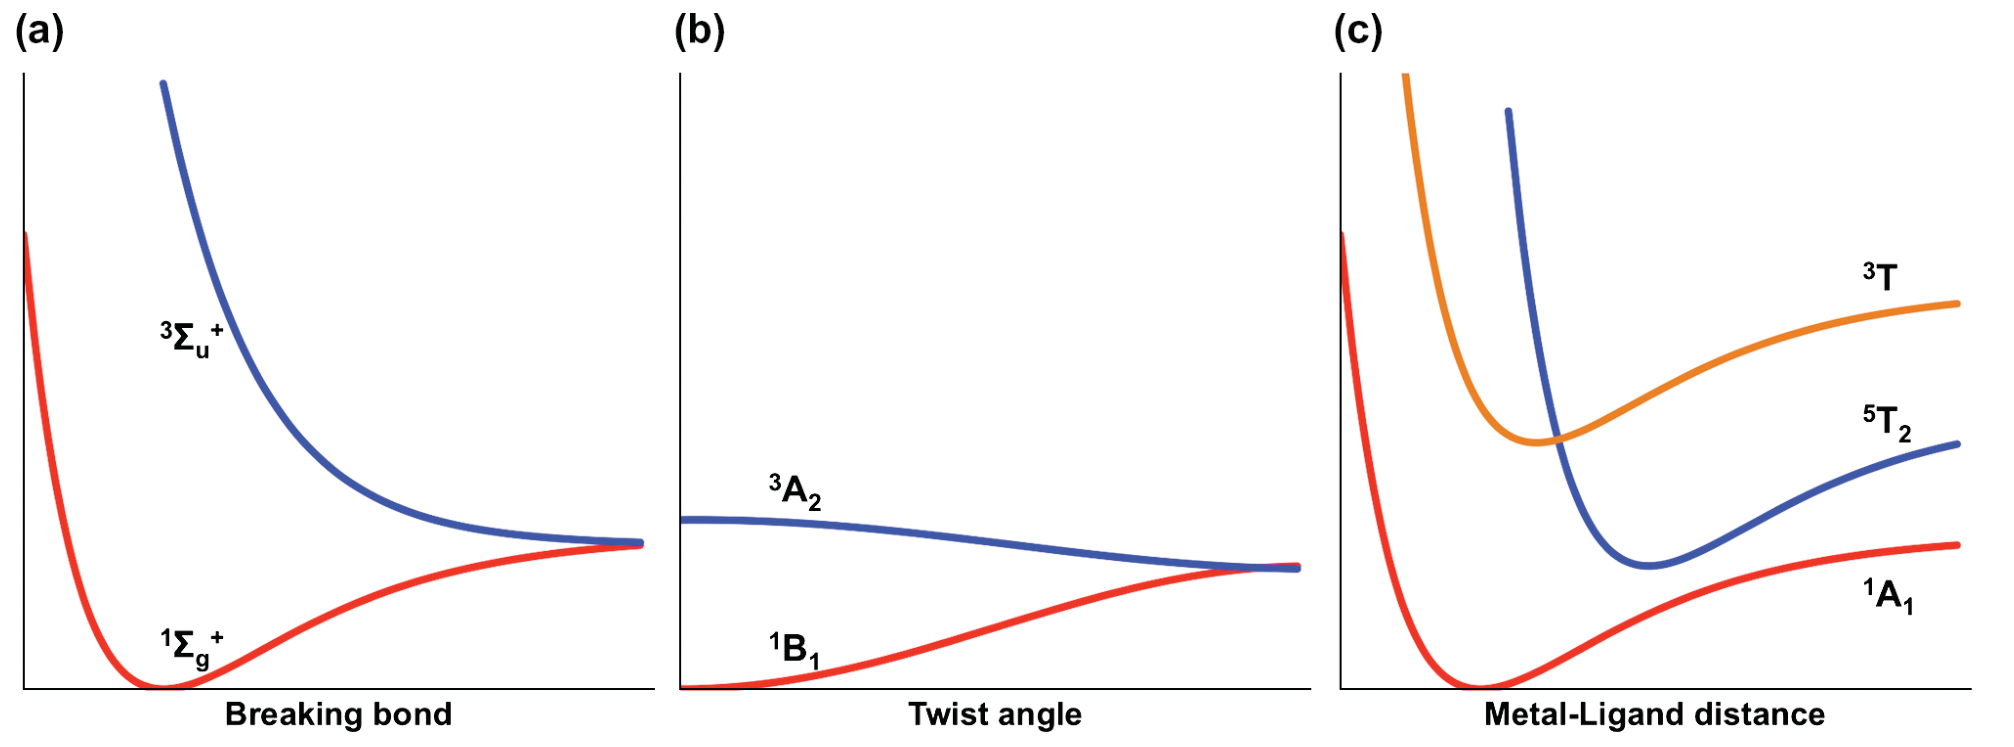
\includegraphics[width=\linewidth]{fig02_state_energies_H2_ethylene_TM.png}
    \vskip0.1cm
    {\scriptsize\cmuted{Fig.\ 2: (a) H$_2$ bond breaking (b) ethylene twist (c) metal--ligand distance}}
  \end{columns}
  \symbolstrip{correlation energy: what a single determinant (Hartree--Fock) misses \quad configuration: one way of filling the orbitals (one
    determinant or spin-adapted combination) \quad term symbols ($^1\Sigma_g^+$, $^3A_2$, \dots): spin multiplicity and spatial symmetry of a state}
\end{frame}

\begin{frame}{H$_2$ in a minimal basis}
  \begin{columns}[c]
    \column{0.55\textwidth}
    one $1s$ function per atom, $\chi_A,\chi_B$, overlap $S$:
    {\begin{align*}
      \sigma_g\equiv\varphi_1&=\frac{\chi_A+\chi_B}{\sqrt{2(1+S)}}\\
      \sigma_u\equiv\varphi_2&=\frac{\chi_A-\chi_B}{\sqrt{2(1-S)}}
    \end{align*}}
    \explain{$\sqrt{2(1\pm S)}$: $\braket{\chi_A\pm\chi_B}{\chi_A\pm\chi_B}=1+1\pm2S$}
    \onslide<2->{\small $\varphi_1$ even, $\varphi_2$ odd under inversion $\Rightarrow$
      $h_{12}=\eri1112=\eri2221=0$}
    \explain<2->{an integral with an odd number of $\varphi_2$'s has an odd integrand: it integrates to zero}
    \column{0.4\textwidth}
    \centering
    \begin{tikzpicture}[scale=0.95]
      \fill[noirgold] (-0.8,0) circle (0.07); \fill[noirgold] (0.8,0) circle (0.07);
      \shade[inner color=noircyan!60,outer color=noirbg] (0,1.4) ellipse (1.5 and 0.55);
      \node[font=\scriptsize,text=noircyan] at (0,2.15) {$\sigma_g$ (bonding)};
      \onslide<2->{
      \shade[inner color=noirrose!60,outer color=noirbg] (-0.95,-1.2) circle (0.5);
      \shade[inner color=noirblue!60,outer color=noirbg] (0.95,-1.2) circle (0.5);
      \draw[noirmuted,dashed] (0,-1.75) -- (0,-0.65);
      \node[font=\scriptsize,text=noirrose] at (0,-2.05) {$\sigma_u$ (antibonding, node)};}
    \end{tikzpicture}
  \end{columns}
  \symbolstrip{$\chi_A,\chi_B$: hydrogen $1s$ atomic orbitals on nuclei $A$, $B$ \quad $S=\braket{\chi_A}{\chi_B}$: their overlap \quad
    $g$/$u$: even/odd under inversion through the bond centre \quad indices 1, 2 below mean $\varphi_1,\varphi_2$}
\end{frame}

\begin{frame}{The $2\times2$ CI problem}
  the OSS ($^1\Sigma_u^+$) is alone; the two closed shells $\sigma_g^2,\sigma_u^2$ ($^1\Sigma_g^+$) mix:
  {\[
    \mathbf H=\begin{pmatrix}E_1&K_{12}\\K_{12}&E_2\end{pmatrix},\qquad E_1=2h_{11}+J_{11}\ (\text{RHF}),\quad E_2=2h_{22}+J_{22}
  \]}
  \explain{the coupling $K_{12}$ is the closed-shell/closed-shell element $\mel{\Phi_{\text i}}{\Hop}{\Phi_{\text{ii}}}$ derived in Part V}
  {\begin{align*}
    \uncover<2->{\det(\mathbf H-E\mathbf 1)}&\uncover<2->{=(E_1-E)(E_2-E)-K_{12}^2=0} &&\uncover<2->{\why{eigenvalue condition}}\\
    \uncover<3->{E^2-(E_1+E_2)E+E_1E_2-K_{12}^2}&\uncover<3->{=0} &&\uncover<3->{\why{multiply out}}\\
    \uncover<4->{E_{\text{CI}}}&\uncover<4->{=\tfrac12\Bigl[E_1+E_2-\sqrt{(E_2-E_1)^2+4K_{12}^2}\Bigr]} &&\uncover<4->{\why{lower root of the quadratic}}
  \end{align*}}
  \onslide<5->{\centering\small also: $E(^3\Sigma_u^+)=h_{11}+h_{22}+J_{12}-K_{12}$,\quad $E(^1\Sigma_u^+)=h_{11}+h_{22}+J_{12}+K_{12}$\par}
  \symbolstrip{CI: configuration interaction (diagonalise $\Hop$ among several configurations) \quad RHF: restricted Hartree--Fock, both electrons in $\sigma_g$
    \quad $^3\Sigma_u^+$, $^1\Sigma_u^+$: the triplet and open-shell singlet of $\sigma_g^1\sigma_u^1$}
\end{frame}

\begin{frame}{Pulling the atoms apart (1/2): the integrals}{assume $R\to\infty$: $S\to0$, every overlap density $\chi_A\chi_B\to0$; \ $U=\eri AAAA$, \ $V=\eri AABB\to1/R$}
  {\begin{align*}
    \varphi_1^2&=\tfrac12(\chi_A^2+\chi_B^2+\canc<2->{2\chi_A\chi_B})\to\tfrac12(\chi_A^2+\chi_B^2) &&\why{the atoms no longer overlap}\\
    \uncover<3->{\varphi_2^2}&\uncover<3->{\to\tfrac12(\chi_A^2+\chi_B^2)} &&\uncover<3->{\why{same, minus sign gone}}\\
    \uncover<4->{\varphi_1\varphi_2}&\uncover<4->{\to\tfrac12(\chi_A^2-\chi_B^2)} &&\uncover<4->{\why{$\tfrac12(\chi_A+\chi_B)(\chi_A-\chi_B)$}}\\
    \uncover<5->{J_{11}=J_{22}=J_{12}}&\uncover<5->{\to\tfrac14\bigl[U+V+V+U\bigr]=\tfrac12(U+V)} &&\uncover<5->{\why{4 cross terms of two $\tfrac12$-clouds}}\\
    \uncover<6->{K_{12}}&\uncover<6->{\to\tfrac14\bigl[U-V-V+U\bigr]=\tfrac12(U-V)} &&\uncover<6->{\why{the $\chi_B^2$ part enters with $-$}}
  \end{align*}}
  \onslide<7->{\centering\small and $h_{11}=h_{22}\to E_H-\tfrac1R$ \ (an electron on A still feels nucleus B as a point charge)\par}
  \symbolstrip{$R$: H--H distance \quad $U$: repulsion of two electrons on the \emph{same} atom \quad $V$: repulsion of electrons on \emph{different} atoms
    ($\to1/R$, two point charges) \quad $E_H$: energy of an isolated H atom}
\end{frame}

\begin{frame}{Pulling the atoms apart (2/2): the energies}
  \begin{align*}
    E_{\text{RHF}}&=2h_{11}+J_{11}+\tfrac1R=2E_H-\tfrac2R+\tfrac U2+\tfrac{V}{2}+\tfrac1R
      \uncover<2->{\overset{V=1/R}{=}2E_H+\hlr<3->{\tfrac U2}-\tfrac1{2R}}\\
    \uncover<4->{E_T}&\uncover<4->{=2h_{11}+J_{12}-K_{12}+\tfrac1R=2E_H-\tfrac2R+V+\tfrac1R\overset{V=1/R}{=}\hlg<5->{2E_H}}\\
    \uncover<6->{E_{\text{CI}}}&\uncover<6->{=E_1-K_{12}\ (E_1=E_2)=2E_H+\tfrac U2-\tfrac1{2R}-\tfrac{U-V}{2}\to\hlg<7->{2E_H}}\\
    \uncover<8->{E(^1\Sigma_u^+)}&\uncover<8->{=E_T+2K_{12}\to2E_H+U-V}
  \end{align*}
  \explain<2->{RHF keeps $U/2$ because half of $\sigma_g^2$ is H$^+$H$^-$; in CI, $E_1=E_2$ so the root is $E_1-K_{12}$, and $K_{12}=\tfrac{U-V}{2}$ cancels it}
  \onslide<9->{\centering\cgreen{RHF misses the dissociation limit by $U/2$; one extra configuration fixes it exactly.}\par}
  \symbolstrip{$2E_H$: the correct limit, two separate H atoms \quad $E_1=2h_{11}+J_{11}$, $E_2=2h_{22}+J_{22}$ become equal as $R\to\infty$}
\end{frame}

\begin{frame}{What the CI wavefunction is}
  at $R\to\infty$ the eigenvector is $c_1=-c_2=\tfrac1{\sqrt2}$ \quad\cgold{(two configurations, equal weight)}
  {\begin{align*}
    \uncover<2->{\varphi_1(1)\varphi_1(2)}&\uncover<2->{=\tfrac12\bigl[\underbrace{\chi_A\chi_B+\chi_B\chi_A}_{\text{covalent}}
      +\underbrace{\chi_A\chi_A+\chi_B\chi_B}_{\text{ionic}}\bigr]} &&\uncover<2->{\why{expand $(\chi_A+\chi_B)^2/2$}}\\
    \uncover<3->{\varphi_1\varphi_1-\varphi_2\varphi_2}&\uncover<3->{=\tfrac12\bigl[(\chi_A+\chi_B)^2-(\chi_A-\chi_B)^2\bigr]} &&\uncover<3->{\why{the CI combination}}\\
    &\uncover<4->{=\chi_A(1)\chi_B(2)+\chi_B(1)\chi_A(2)} &&\uncover<4->{\why{ionic terms cancel}}
  \end{align*}}
  \onslide<5->{\centering
  \begin{tikzpicture}
    \node[draw=noirrose,rounded corners,fill=noirpanel,inner sep=5pt,align=center,font=\small] at (0,0)
      {RHF: 50\% ionic\\ H$^+$H$^-$ at infinity costs $U/2$};
    \node[draw=noirgreen,rounded corners,fill=noirpanel,inner sep=5pt,align=center,font=\small] at (6,0)
      {CI: purely covalent\\ Heitler--London H$\cdot$ $\cdot$H};
  \end{tikzpicture}\par}
  \symbolstrip{covalent: one electron on each atom \quad ionic: both electrons on one atom (H$^-$ next to H$^+$) \quad
    $c_1,c_2$: CI coefficients of $\sigma_g^2$ and $\sigma_u^2$ (shorthand $\chi_A\chi_B\equiv\chi_A(1)\chi_B(2)$)}
\end{frame}

\begin{frame}{H$_2$ curves from our calculation}{STO-3G, PySCF; closed forms agree to $4\times10^{-16}\,\Eh$ (T5)}
  \centering
  \begin{tikzpicture}
    \begin{axis}[noirplot,width=11.5cm,height=5.2cm,xmin=0.8,xmax=8,ymin=-1.2,ymax=0.2,
        xlabel={$R$ (bohr)},ylabel={$E$ ($\Eh$)},legend pos=south east,legend columns=2,ymajorgrids]
      \addplot[noirmuted,dashed,thick] table[x=R,y=twoEH,col sep=comma]{data/h2_curves.csv};
      \addlegendentry{$2E_H$}
      \only<1->{\addplot[noirgold,very thick] table[x=R,y=RHF,col sep=comma]{data/h2_curves.csv};}
      \addlegendentry{RHF}
      \only<2->{\addplot[noircyan,very thick] table[x=R,y=CI,col sep=comma]{data/h2_curves.csv};}
      \only<2->{\addlegendentry{CI $=$ FCI ($^1\Sigma_g^+$)}}
      \only<3->{\addplot[noirrose,very thick] table[x=R,y=T,col sep=comma]{data/h2_curves.csv};}
      \only<3->{\addlegendentry{triplet $^3\Sigma_u^+$}}
      \only<4->{\addplot[noirblue,very thick] table[x=R,y=OSS,col sep=comma]{data/h2_curves.csv};}
      \only<4->{\addlegendentry{OSS $^1\Sigma_u^+$}}
    \end{axis}
  \end{tikzpicture}
  \vskip-0.1cm
  \onslide<3->{\small CI and triplet converge on $2E_H$; RHF does not (T5: still $0.362\,\Eh=K_{12}$ too high at $R=20$ bohr)}
  \symbolstrip{STO-3G: minimal Gaussian basis (one $1s$ function per H) \quad FCI: full CI, exact in this basis \quad
    bohr $=0.529$\,\AA \quad $2E_H=-0.9332\,\Eh$ in STO-3G}
\end{frame}

\begin{frame}{The general rule: orbital gap versus exchange}
  \begin{columns}[c]
    \column{0.48\textwidth}
    model: $h_a=-\tfrac\Delta2$, $h_b=+\tfrac\Delta2$, $J_{aa}=J_{bb}=J_d$, $J_{ab}=J_x$
    {\begin{align*}
      \uncover<2->{\mathbf H}&\uncover<2->{=\begin{pmatrix}J_d-\Delta&K\\K&J_d+\Delta\end{pmatrix}}\\
      \uncover<3->{E_S}&\uncover<3->{=J_d-\sqrt{\Delta^2+K^2}}\\
      \uncover<4->{\frac{c_2}{c_1}}&\uncover<4->{=\frac{\Delta-\sqrt{\Delta^2+K^2}}{K}}\\
      \uncover<5->{E_S-E_T}&\uncover<5->{=(J_d-J_x)+K-\sqrt{\Delta^2+K^2}}
    \end{align*}}
    \explain<2->{diagonal $2h+J$; $E_S$ is the lower root; $c_2/c_1$ from row 1, $(J_d-\Delta-E_S)c_1+Kc_2=0$; $E_T=J_x-K$}
    \column{0.5\textwidth}
    \onslide<4->{
    \begin{tikzpicture}
      \begin{axis}[noirplot,width=6.2cm,height=4.4cm,xmin=0,xmax=6,ymin=-1.05,ymax=0.05,
          xlabel={$\Delta/K$},ylabel={$c_2/c_1$},ymajorgrids]
        \addplot[noircyan,very thick,domain=0:6,samples=80] {x-sqrt(x^2+1)};
        \node[font=\scriptsize,text=noirrose,anchor=west] at (axis cs:0.15,-0.9) {diradical: equal weights};
        \node[font=\scriptsize,text=noirgreen,anchor=east] at (axis cs:5.9,-0.2) {closed shell};
      \end{axis}
    \end{tikzpicture}}
    \onslide<6->{\small\okpill\ weak interaction $\Rightarrow$ strong static correlation (T6)}
  \end{columns}
  \symbolstrip{Fig.\ 2b: twisting ethylene to $90^\circ$ closes the $\pi$/$\pi^*$ gap ($\Delta\to0$; standard result) \quad $\Delta=h_b-h_a$ \quad $J_d$: same-orbital repulsion, $J_x$: different-orbital
    \quad $c_2/c_1=-1$: two configurations of equal weight (a pure diradical); $\to0$: one configuration}
\end{frame}
